\documentclass[12pt]{article}

\usepackage[parfill]{parskip}
%INSERT IMAGE
\usepackage{float}
\usepackage{graphicx}

\begin{document}

\begin{titlepage}

\newcommand{\HRule}{\rule{\linewidth}{0.5mm}} % Defines a new command for the horizontal lines, change thickness here

\center % Center everything on the page
 
%----------------------------------------------------------------------------------------
%	HEADING SECTIONS
%----------------------------------------------------------------------------------------

\textsc{\Large University of Applied Sciences Bonn Rhein Sieg}\\[0.4cm] % Name of your university/college
\textsc{\Large R\&D Proposal}\\[0.5cm] % Major heading such as course name
%\textsc{\large Minor Heading}\\[0.5cm] % Minor heading such as course title

%---------------------------------------------------------------------------------------
%	TITLE SECTION
%----------------------------------------------------------------------------------------

\HRule \\[0.4cm]
{ \large eTa: Evolutionary Optimization of a Wheel Hub Motor}\\[0.01cm] % Title of your document
\HRule \\[1.5cm]
% Object recognition as a service
% OR library/tool 
% OR tool based on SC and DL
% OR tool based on SC and DL for service robotics
% DL OR tool for service robotics
% DL OR tool for service robotics developers
% OR with DL and SC : A tool for robotics developers
% OR based on DL and SC : A tool with tuning and training assistance
% DL with SC OR : A tool with training and tuning assistance
 
%----------------------------------------------------------------------------------------
%	AUTHOR SECTION
%----------------------------------------------------------------------------------------

\begin{minipage}{0.4\textwidth}
\begin{flushleft} \large
\emph{Author:}\\ [0.0cm]
Bastian \textsc{Lang}\\ [0.0cm] % Minor heading such as course title% Your name
\small{ Matrikel Nr. 90345674} \\ [0.0cm]
\footnotesize{ bastian.lang@smail.inf.h-brs.de}
\end{flushleft}
\end{minipage}
~
\begin{minipage}{0.5\textwidth}
\begin{flushright} \large
\emph{Advisors:} \\ [0.0cm]
Prof. Dr. Alexander \textsc{Asteroth} \\ % Supervisor's Name
Dr. Nils \textsc{Bornemann}
\end{flushright}
\end{minipage}\\[4cm]

% If you don't want a supervisor, uncomment the two lines below and remove the section above
%\Large \emph{Author:}\\
%John \textsc{Smith}\\[3cm] % Your name

%----------------------------------------------------------------------------------------
%	DATE SECTION
%----------------------------------------------------------------------------------------

{\large \today}\\[3cm] % Date, change the \today to a set date if you want to be precise

%----------------------------------------------------------------------------------------
%	LOGO SECTION
%----------------------------------------------------------------------------------------

%\includegraphics{Logo}\\[1cm] % Include a department/university logo - this will require the graphicx package
 
%----------------------------------------------------------------------------------------

\vfill % Fill the rest of the page with whitespace
\end{titlepage}

\section{Introduction}

During the last two years GKN Sinter Metals has developed a new transverse flux motor.
That is a high performance electric motor with size, weight, performance and efficiency advantages when compared to traditional electric motors[1].

The motor has been constructed from SMC powder using additive manufacturing (3D printing).
Even small sized such motors are capable of producing a high torque.
The current that is needed to produce such high torque produces a great amount of heat, which needs to be dissipated.

For the heat dissipation the motor's casing plays a central role.
The current design of the casing (see figure \ref{fig_casing}) has been manually optimized using a detailed model of the motor's thermodynamic properties.

\begin{figure}
	\centering
  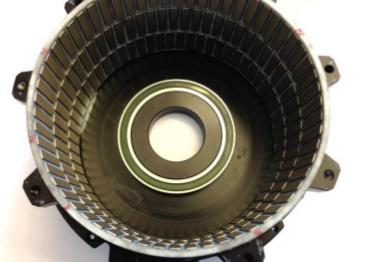
\includegraphics[width=0.4\textwidth]{images/rotor.jpg}
	\caption{Rotor of transverse flux motor.}
	\label{fig_casing}
\end{figure}

Because of the infinitely high number of possible designs there is a high chance that there are more optimal designs with respect to heat dissipation and motor weight.

\section{Goal}
The objective of this R\&D is to design a (more) optimal casing for the transversal flux motor with respect to heat dissipation, weight and structural integrity.
To achieve this objective, Evolutionary Algorithms (EAs) will be used.

\begin{figure}
	\centering
  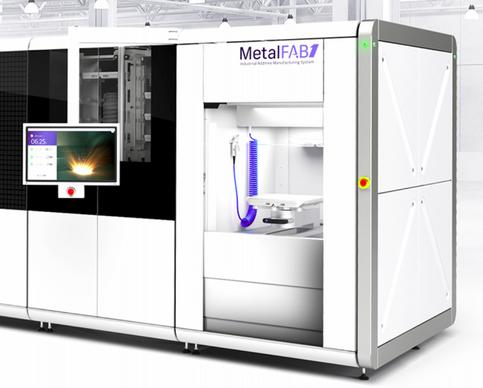
\includegraphics[width=0.4\textwidth]{images/printer.jpg}
	\caption{Device for additive manufacturing at GKN Sinter Metals}
	\label{fig_additive}
\end{figure}


Initially the thermodynamic model of the motor will be kept simple and a first attempt will only optimize the design for heat dissipation.

In a later stage of the project the design will be optimized not only for heat dissipation, but for weight and structural integrity as well.

Once a good solution has been found in simulation, a prototype will be produced and evaluated in the real world.


\section{Approach}
\subsection{Thermodynamic Model}
The initial thermodynamic model of the motor will assume a constant, uniform heat source. 
This will probably encourage a symmetric solution for the design of the casing, because the heat emission will be the same.
A more complex and realistic model of the motor will be used in a later approach once the first attempt was successful.

\subsection{Representation}
The algorithm will optimize the 3D shape of the casing, i.e. the 3D representation of the shape. 
EAs such as CMA-ES work best at a parameter count of about 40.
This creates the need of finding a concise representation of the 3D shape.
Splines could be one way of addressing this problem.
Assuming a symmetric solution, it would not be necessary to model the whole shape, but only a small part of it.
Maybe even a transformation of the problem into 2D and a later retransformation could provide important insights.

\subsection{Evolutionary Algorithms}
As a first attempt a single objective EA such as CMA-ES\cite{hansen2001completely} or alike will be used to optimize for the heat dissipation.
Once this has been done successfully, multi-objective algorithms such as NSGA-II\cite{deb2002fast} will be applied to account for weight and structural integrity as well.
Starting simple will help to focus on problems regarding the representation and simulation first before going on to more complex algorithms.

\subsection{Expected Results}
\begin{itemize}
\item \textbf{Minimum}
\begin{itemize}
	\item Comprehensive literature research of current research in this area and available technology
	\item Parameterized 3D design of model
	\item Implementation of simplified thermal motor model
	\item Optimization of 3D model's parameters w.r.t. heat dissipation using one evolutionary method
\end{itemize}

\item \textbf{Expected}
\begin{itemize}

	\item Optimization for multiple objectives (dissipation, weight, structure)
	\item 3D printed design
	
\end{itemize}

\item \textbf{Maximum}
\begin{itemize}
	\item Optimization using more realistic model (e.g. including multiple, located heat sources, air flow)
	\item Thorough evaluation of above also in real world
\end{itemize} 
\end{itemize}

\section{Project Plan}
\subsection{Workpackages}
\begin{itemize}
	\item \textbf{Knowledge in Motor Technology and Simulation}
	\begin{itemize}
		\item Literature research
		\item Find related work
	\end{itemize}

	\item Simulation
	\begin{itemize}
		\item Evaluate Matlab frameworks for thermodynamic simulation
		\item Create simple thermodynamic motor model 
	\end{itemize}

	\item Representation
	\begin{itemize}
		\item Evaluate ways to parameterize 3D shapes of the motor
	\end{itemize}		
	
	\item Single Objective Optimization
	\begin{itemize}
		\item Literature Research on EAs
		\item Choose and Implement EA
		\item Evolve Design w.r.t. Heat Dissipation using Simple Model
	\end{itemize}
	
	\item Multi Objective Optimization
	\begin{itemize}
		\item Literature Research on Multi Objective EAs
		\item Choose and Implement MO-EA
		\item Evolve Design w.r.t. Heat Dissipation, Weight and Structure using Simple Model
	\end{itemize}
	
	\item Real World Evaluation
	\begin{itemize}
		\item Produce Prototype
		\item Evaluate Prototype
	\end{itemize}
	
\end{itemize}

\newpage
\nocite{*}
\bibliographystyle{abbrv}
\bibliography{literature.bib}



\end{document}
